\MindQuantum\ places great emphasis on the simulation efficiency of NISQ algorithms, particularly variational quantum algorithms. In this study, we benchmarked \MindQuantum\ against other mainstream quantum computing frameworks. Firstly, we used random circuit simulation to benchmark the fundamental performance of the framework. Secondly, we used Quantum Approximate Optimization Algorithm (QAOA) for benchmarking, demonstrating MindQuantum’s ability to solve practical problems. The table below shows the frameworks that participated in the benchmark.

\begin{table}[ht]
    \begin{tabular}{cc}
        \toprule
        Framework           & Version       \\
        \midrule
        MindQuantum         & 0.9.0         \\
        Qiskit              & 0.45.0        \\
        Qulacs              & 0.6.2         \\
        Tensorflow Quantum  & 0.7.2         \\
        Intel-QS            & 2.0.0-beta    \\
        QuEST               & 3.7.0         \\
        \bottomrule
    \end{tabular}
    \caption{The software version of benchmarking.}
    \label{tab:software version}
\end{table}

The hardware platform used for the benchmark test is Intel® Xeon® CPU E5-2690 v3 @ 2.60GHz, with 8 CPUs and 32G memory, with SIMD enabled. The GPU model is NVIDA-V100.

\subsection{Running Random Circuit Task}

To optimize testing time, we employ the formula $40 \times (4−n)+1000$ to determine the number of gates in circuit, where $n$ represents the number of qubits. We use random circuit sampling with 4-24 qubit scales to evaluate the performance of circuit evolution. The random circuit comprises single-qubit gates X, Y, Z, H, S, T, two-qubit gates CX, CY, CZ, single-qubit parameterized gates RX, RY, RZ, and two-qubit parameterized gates Rxx, Ryy, Rzz. To minimize accidental errors, the final result is obtained by averaging multiple samples.

\begin{figure*}[htbp]
    \begin{center}
        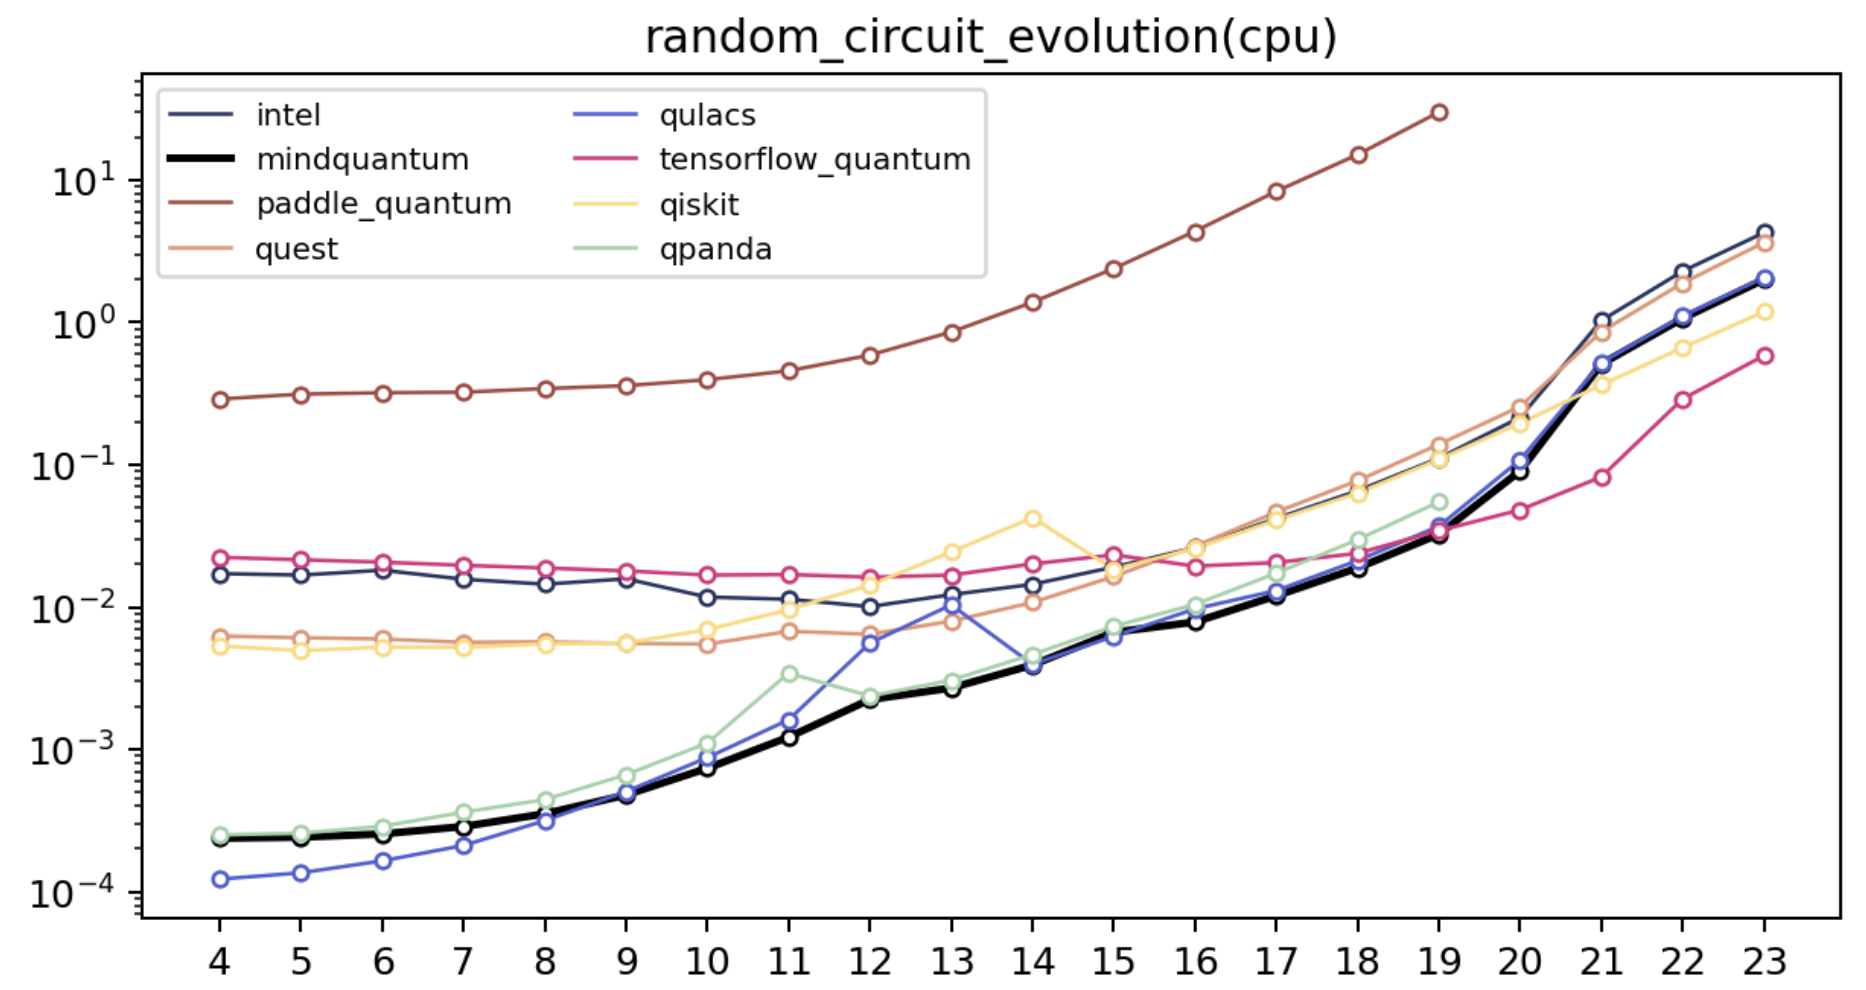
\includegraphics[width=0.7\linewidth]{7_figures/random_circuit_CPU.png}
    \end{center}
    \caption{random circuit CPU}
\end{figure*}

In general, the simulation time increases exponentially with the circuit scale. However, when the number of qubits is small, \MindQuantum, Qulacs and Qpanda have a clear advantage in terms of time compared to other frameworks, which is due to small overhead. It is worth noting that there is a slight dip at the 13-qubit position because \MindQuantum\ uses 13 qubits as a threshold, and when the number of qubits is greater than 13, it enables OpenMP to perform multi-threaded parallel computing. This is because we found that multi-threaded computing would reduce the running speed when the number of qubits is small. As the circuit scale continues to increase, \MindQuantum\ and Qulacs maintain a good speed advantage, which can be judged that the two frameworks have been optimized to near the limit at the low-level implementation. However, Tensorflow Quantum eventually surpassed them. We analyzed that the reason may be that Tensorflow’s parallel computing strategy is more advanced, which makes it more advantageous in simulating large-scale quantum systems.

\subsection{QAOA Task}

Now, we use Quantum Approximate Optimization Algorithm for benchmarking, which can further demonstrate the performance of the framework in solving practical problems. We apply QAOA to find the max-cut of 4-regular graphs and fully connected graphs, covering the cases of low and high entanglement. The size of the problem ranges from 5 to 22 nodes. The ansatz circuit is obtained by one-step Trotter decomposition. The optimizer is \code{scipy.optimize.minimize()} with the BFGS method.

\begin{figure*}[htbp]
    \begin{center}
        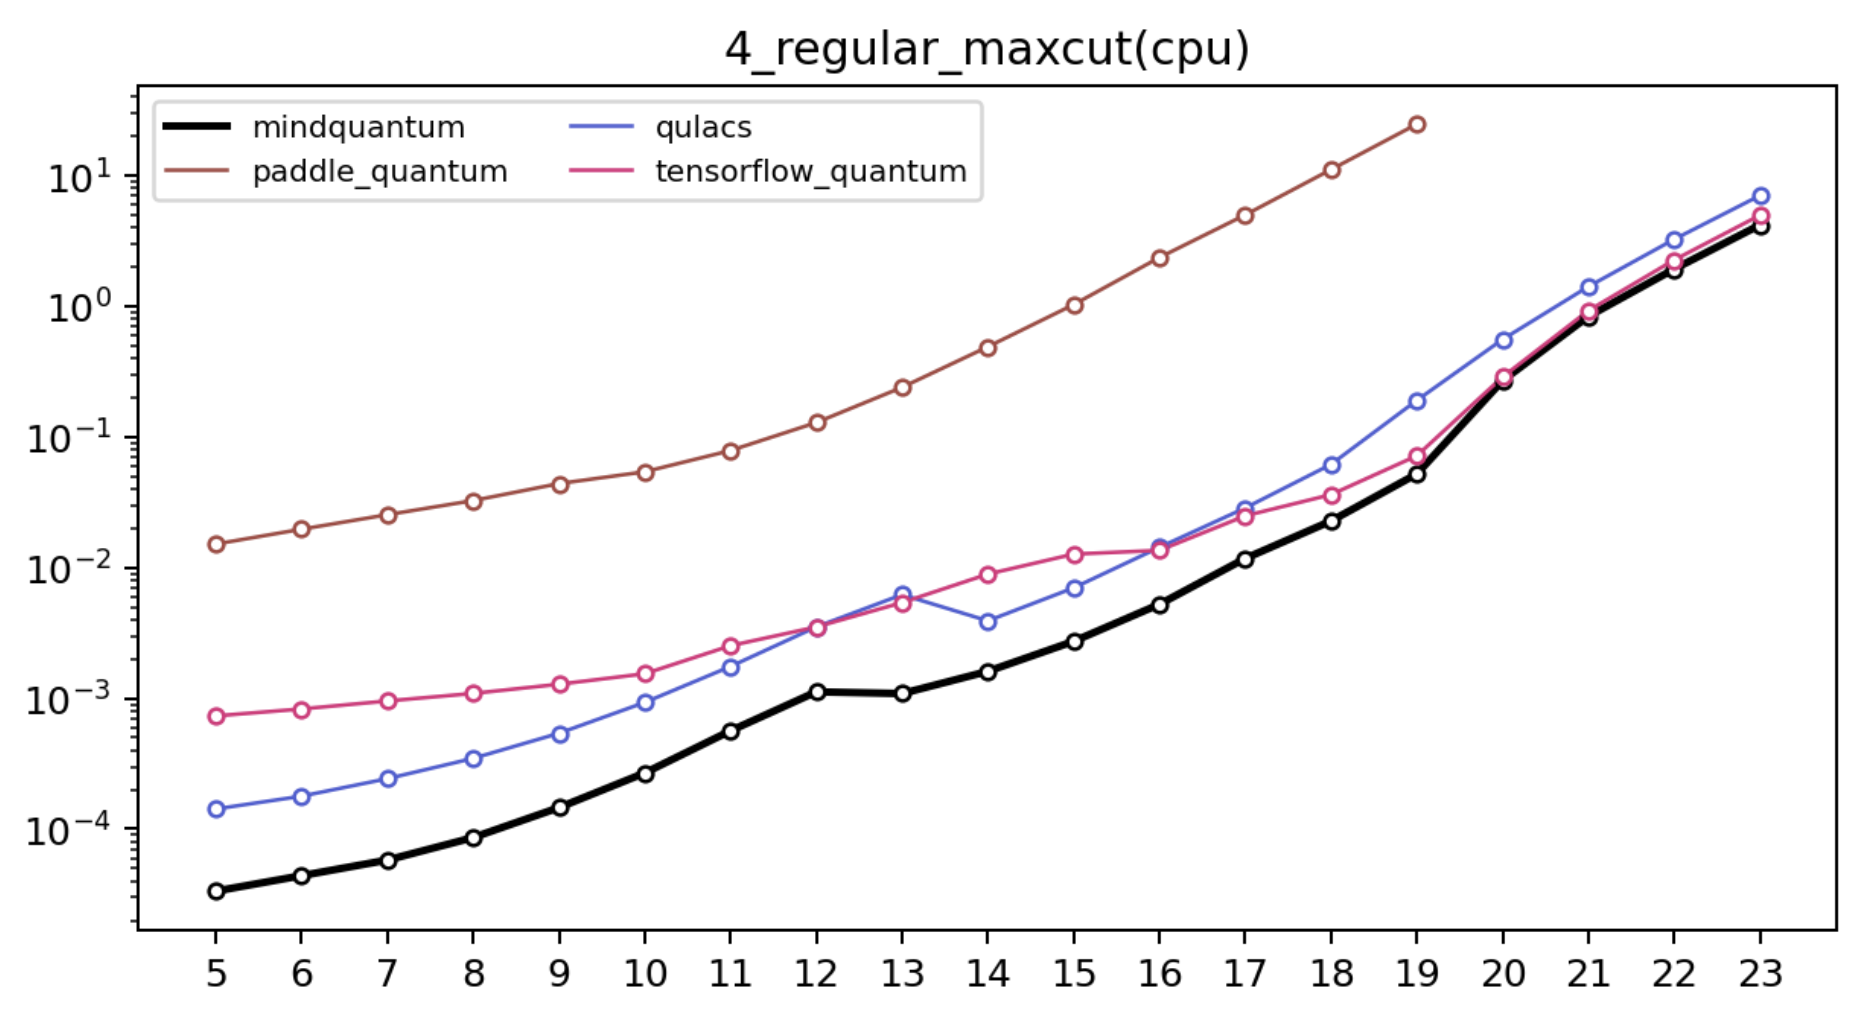
\includegraphics[width=0.7\linewidth]{7_figures/4_regular_CPU.png}
    \end{center}
    \caption{4 regular maxcut CPU}
\end{figure*}

Overall, as the problem size increases, the solution time of all frameworks grows exponentially. However, \MindQuantum\ is one orders of magnitude faster than other frameworks for problems with less than 16 qubits, and it also reaches the best performance for larger qubit numbers. This is mainly due to MindQuantum’s many targeted optimizations for getting parameter gradient steps and efficient implementation of circuit evolution.